\chapter{Final Source-Corrected Results}
\label{ch:results}

\section{Evidence basis}

All values in this chapter come from the source-corrected complete-case full-population analysis artifact, version \texttt{source-corrected-complete-case-full-population-analysis-v2}, SHA-256 \artifacthash. The evidence selection is explicit because earlier historical lineages are retained for auditability but are comparison-only. No new provider requests were performed to calculate the values reported here.

\section{RQ1: agreement with human preference reference labels}

Across 772 analytical observations, judges exactly matched the human preference reference label in 457 cases, an agreement rate of 59.20\% (95\% CI 55.70--62.69\%). Cohen's $\kappa$ was 0.3230 (95\% CI 0.2698--0.3758). This is a moderate association in the practical sense that agreement is visibly above a naive random baseline but far from universal. The result must not be rephrased as ground-truth accuracy: human preference labels are the stated reference and can contain task- and annotator-dependent judgements.

The descriptive per-judge rates show heterogeneity: Claude 45.45\% (85/187), DeepSeek 67.55\% (127/188), GPT 57.00\% (114/200), and Llama 66.50\% (131/197). These numbers are not a global model ranking. They arise within this controlled dataset, protocol, validity policy, and human-label population.

\section{RQ2: repeated-evaluation consistency}

The strict complete repeated-evaluation result is 96.53\% (7,119/7,375 valid repeated decisions) across 1,475 strict valid cells. A conditional sensitivity analysis reports 96.31\% over 1,585 cells. Physical completeness was 1,599/1,600 cells. Thus the protocol was highly repeatable under its fixed condition, with transparent missingness rather than forced completion. This result does not contradict RQ3: a judge may repeat a decision reliably when shown the same prompt and still react differently when the answer order changes.

\section{RQ3: position sensitivity}

Among 799 physical AB/BA pairs, 759 were valid paired outcomes and 549 were decisive after mapping decisions back to original answer identities. There were 96 decisive mapped flips, giving a primary flip rate of 17.49\%. The broader all-paired outcome disagreement rate was 193/759 = 25.43\%. The gap between these values reflects the distinction between a decisive winner reversal and any mapped outcome difference, including ties.

Per-judge decisive flip rates were Claude 53.70\% (58/108), DeepSeek 10.98\% (19/173), GPT 2.70\% (3/111), and Llama 10.19\% (16/157). This is an empirical position-sensitivity observation within the experiment; it does not identify a causal internal mechanism or license a general statement about future model versions.

\section{RQ4 and RQ5: narrow controlled treatments}

RQ4 found zero stable redundant-text variant wins among 682 eligible pairs (0.00\%). RQ5 found zero stable presentation/list-prefix variant wins among 716 eligible pairs (0.00\%). Both results are clear for the specified frozen treatments and eligible denominators. They should not be turned into broad claims that longer answers, verbose answers, or all formatting changes do not influence language-model judges. The point of these experiments is to make the treatment sufficiently narrow that the inference is honest.

\section{RQ6: matched source-family preference}

The counterbalanced source-family result is 81/159 = 50.94\% stable same-family preference (95\% CI 42.77--58.49\%), with 33.13\% coverage from 159 of 480 planned units. The aggregate interval includes 50\%. Judge-specific descriptive rates vary strongly: Claude 25/29 = 86.21\%, GPT 50/66 = 75.76\%, and Llama 6/64 = 9.38\%. The evidence therefore does not support a uniform overall same-family preference claim. It supports an observed association in the counterbalanced protocol with strong judge-level heterogeneity and limited stable-decisive coverage.

\section{RQ7: mitigation trade-offs}

For primary DUAL\_SWAP, 799 of 800 linked triplets were physically complete and 597 were retained for the matched agreement comparison. Baseline agreement was 405/597 = 67.84\%; DUAL\_SWAP agreement was 409/597 = 68.51\%. The matched change was +0.67 percentage points with a 95\% CI of -0.17 to +1.68 points. Baseline coverage was 774/799 = 96.87\%, while DUAL\_SWAP coverage was 606/799 = 75.84\%, a -21.03 point change. The appropriate reading is a small, uncertain agreement change paired with a material coverage trade-off.

For secondary strict Multi-Judge Consensus, 1,125 of 1,611 planned pairs were retained (69.83\% coverage). Consensus agreement with human preference reference labels was 808/1,125 = 71.82\%, compared with 66.80\% for the equal-weight individual-judge comparator on the same retained pairs. The matched difference was +5.02 points (95\% CI +4.16 to +5.89). This supports the limited claim that, under this frozen strict four-judge consensus protocol and its own comparator, aggregation increased reference-label agreement on retained pairs. It does not establish superiority over DUAL\_SWAP because the units, comparator, and retained population differ.

\begin{table}[H]
\centering
\caption{Final primary results. Percentages are reported with their frozen analytical denominators.}
\label{tab:primary-results}
\begin{tabularx}{\textwidth}{@{}p{0.10\textwidth}X r X@{}}
\toprule
RQ & Final result & N & Cautious interpretation\\
\midrule
RQ1 & 59.20\% agreement; $\kappa=.3230$ & 772 & agreement with human preference reference labels\\
RQ2 & 96.53\% strict consistency & 1,475 cells & fixed-condition repeatability\\
RQ3 & 17.49\% decisive mapped flips & 549 & answer order can change a decisive result\\
RQ4 & 0.00\% redundant-variant wins & 682 & no stable win in this frozen treatment\\
RQ5 & 0.00\% format-variant wins & 716 & no stable win in this frozen treatment\\
RQ6 & 50.94\% same-family preference & 159 & no uniform aggregate preference; heterogeneous\\
RQ7 DUAL\_SWAP & +0.67 pp agreement; -21.03 pp coverage & 597 & small uncertain gain; lower coverage\\
RQ7 Multi-Judge & +5.02 pp agreement; 69.83\% coverage & 1,125 & secondary within-own-comparator effect\\
\bottomrule
\end{tabularx}
\end{table}

\begin{figure}[H]
\centering
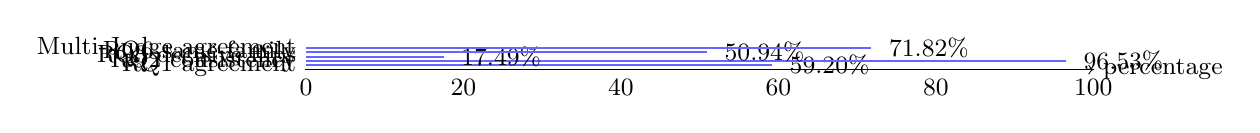
\begin{tikzpicture}[x=1cm,y=0.055cm,font=\small]
\draw[->] (0,0)--(10,0) node[right]{percentage};
\foreach \x/\lab in {0/0,2/20,4/40,6/60,8/80,10/100} \draw (\x,0.1)--(\x,-0.1) node[below]{\lab};
\foreach \y/\lab/\val in {1/RQ1 agreement/59.20,2/RQ2 consistency/96.53,3/RQ3 decisive flips/17.49,4/RQ6 same-family/50.94,5/Multi-Judge agreement/71.82} {\node[left] at (0,\y) {\lab}; \fill[blue!60] (0,\y-0.22) rectangle (\val/10,\y+0.22); \node[right] at (\val/10+0.1,\y) {\val\%};}
\end{tikzpicture}
\caption{Selected final percentages. Metrics measure different estimands and are not a common score or ranking.}
\label{fig:selected-results}
\end{figure}

\begin{figure}[H]
\centering
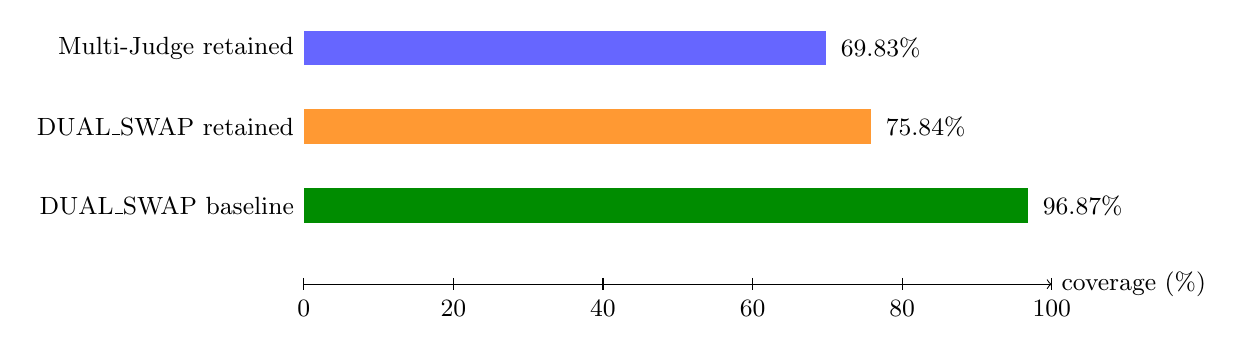
\begin{tikzpicture}[x=0.095cm,y=1cm,font=\small]
\draw[->] (0,0)--(100,0) node[right]{coverage (\%)};
\foreach \x in {0,20,40,60,80,100} \draw (\x,0.08)--(\x,-0.08) node[below]{\x};
\node[left] at (0,1) {DUAL\_SWAP baseline}; \fill[green!55!black] (0,0.78) rectangle (96.87,1.22); \node[right] at (97.5,1) {96.87\%};
\node[left] at (0,2) {DUAL\_SWAP retained}; \fill[orange!80] (0,1.78) rectangle (75.84,2.22); \node[right] at (76.5,2) {75.84\%};
\node[left] at (0,3) {Multi-Judge retained}; \fill[blue!60] (0,2.78) rectangle (69.83,3.22); \node[right] at (70.5,3) {69.83\%};
\end{tikzpicture}
\caption{Coverage is part of the RQ7 mitigation result. The methods use different retained populations and comparators.}
\label{fig:coverage}
\end{figure}
